
\documentclass[article,a4paper]{IEEEtran}
\usepackage{lipsum}
\usepackage[backend=biber]{biblatex}
\usepackage{graphicx}

\addbibresource{refs.bib}
\title{Building Smarter Homes with IoT: Harnessing MQTT, Zigbee, and LoRa}
\author{
\IEEEauthorblockN{Anton Odén}\\
\IEEEauthorblockA{Dept. of Maths and Computer Science\\Karlstad University\\
651 88 KARLSTAD, Sweden}\\
anton.oden@outlook.com
}

\begin{document}

\maketitle

    \begin{abstract}
        
    \end{abstract}

    \section{Introduction}

    \section{Background}
    Communication in IoT is dependent on wireless communication, cause to connect all things by wire would quickly cover much of our space with wires and our wire-bill would match if not superseed the remaining infrastructure. Wireless communicaion could better be described as radio signals. Radio signals communicate at a frequency to avoid collision between different radio signals rules has been applied to what application could use what frequency. Thought these rules could vary globally the ISM-bands different frequencies does has a globally ok coverage making which made is easier to produce communication hardware. For commercial usage different parts of the ISM-band has been opened/allowed to be used \cite{ISM-band1} and the most common commercial standard today in homes, offices, cafés etc. is IEEE 802.11, containing the commonly known WiFi protocol. Communicating at 2400-2483MHz (ISM-band), 5150-5350MHz, 5470-5725 (RLAN, EU standard EN 301 893) and newly introduced 5945-6425MHz (RLAN, EU standard EN 303 687) in WiFi 7 within Europe. \cite{ISM-bandEUR}. Starting from 2.4GHz in 1997 different frequencies bands has been added to satisfy our "desperate" need to high resolution video streaming. 
    \newline\newline
    One problem for IoT end devices that could be running on battery is that WiFi in its aim to give the user high data rate is power consuming. WiFi is designed for high bandwidth or range that results in higher power consumption and for this reasons, new standards has been introduced to IEEE 802 family. 
    \newline\newline
    IEEE 802.15.4, which goes under the name Low-Rate Wireless Personal Area Network (LR-WPAN) is written with low power consumption in mind. The standard is grandfather of protocols such as Zigbee, 6LoWPAN, Thread, SNAP etc. Zigbee was first drafted 2004 and has became famous for usage in smart home implementations. It communicates at the 2400-2483MHz, which is same as WiFi. Also 868-868MHz in Europe and 902-928MHz in North America. Why the split between europe and north america may be Europe having more military applications communicating on 902-928MHz bandwidth \cite{ISM-bandEUR}. Getting the extra communication spectrums makes it easier for the protocol to communicate in highly density Wifi areas. 
    \begin{figure}
        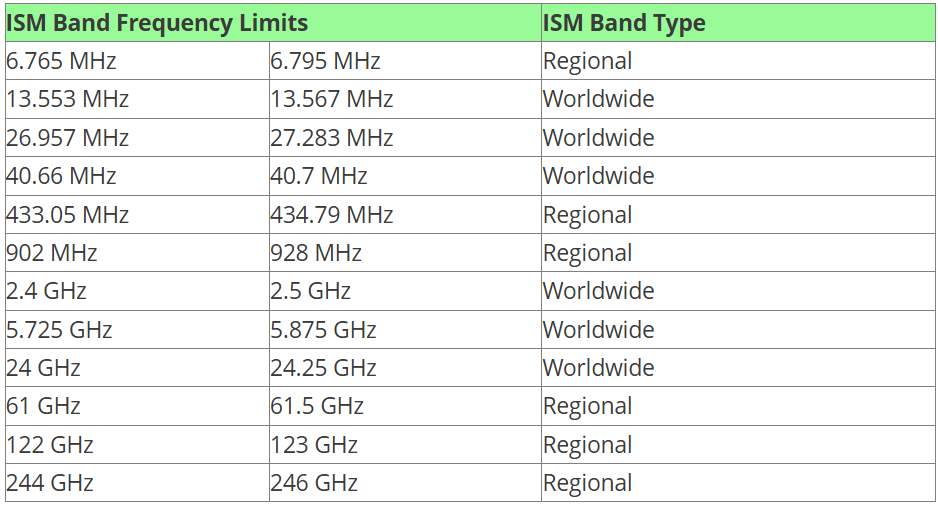
\includegraphics[width=\columnwidth]{ISM-band.png} 
        \caption{ISM-band frequency limits from \cite{ISM-band1}}
        \label{fig1:ISM-band frequency limits}   
    \end{figure}
    \ref{fig1:ISM-band frequency limits}
    Units within a zigbee network are categoriesed into three types. Coordinator, routers and end devices. The routers could be and often are an end device at the same time. The routers extend the physical range of the network and makes the network reliability as if one router goes offline the network so communication is not broken. This presupposes that end devices has more than one router in reachable range that can reach other parts of the network. The term mesh network is coined describing a zigbee network thought the network could also be structured in a star or tree topology also. "Mesh network: This is a network in which the routing of messages is performed as a decentrilized, cooperative proces involving many peer devices routing on each other's behalf." \cite{ZigbeeSpec}. So the routing devices are enabler of mesh network. The coordinator is only one within the personal area network and it is responsible of adding and decoupling devices to the network and the coordinator must be a fully functional device. End devices are all the things we want to connect in our IoT, usually a sensor/measuring instrument or some kind of actuator. 
    \newline\newline
    To add functionality to the network another protocol is needed on top of Zigbee, as Zigbee is used for the communication. The most famous protocol for this is Message Queue Telemetry Transport (MQTT). MQTT filters all messages in a publish/subscribe manor. So MQTT terminology divide the network up in MQTT broker and MQTT clients, where the MQTT broker serves at the central hub in the messaging system. All clients connected to the MQTT broker published messages to the broker, all published messages are labeled with a topic (usally friendly devicename for sensor IoT devices). All clients in the MQTT network can subscribe to specified published topics. So for example if an IRsensor send/publish a message with topic "AwesomeRobotSolutionIRSensor", all clients that are subscribing to topic "AwesomeRobotSolutionIRSensor" will recieve the published message via the MQTT broker.       
    \section{The Challenges of Smart Home Networking}

    \section{Why Combine MQTT, Zigbee, and LoRa?}

    LorAWAN
    1. 

    \section{Designing the Network Architecture}

    \section{Practical Use Cases}

    \section{Future Trends and Innovations}

    \section{Conclusion}

\printbibliography

\end{document}